\section{Design}
\label{sec:Design}

\subsection{Overview} 
NeuraViz follows a fairly standard server-client web application architecture. The client is responsible for rendering the user interface and allowing the user to interact with the application. The server handles the actual computationally intensive processes such as parsing the uploaded model and generating the structure of the visual representation. The server also handles the storage of the uploaded models during user sessions. It also handles translation of the visualization into various formats.

\subsection{UML Class Diagram}
The UML class diagram in Figure \ref{fig:uml_class_diagram} shows the classes and their relationships in the NeuraViz application. The diagram is divided into two main sections: the frontend and the backend, which are also commonly referred to as the client and server respectively. 

\begin{figure}[h]
    \centering
    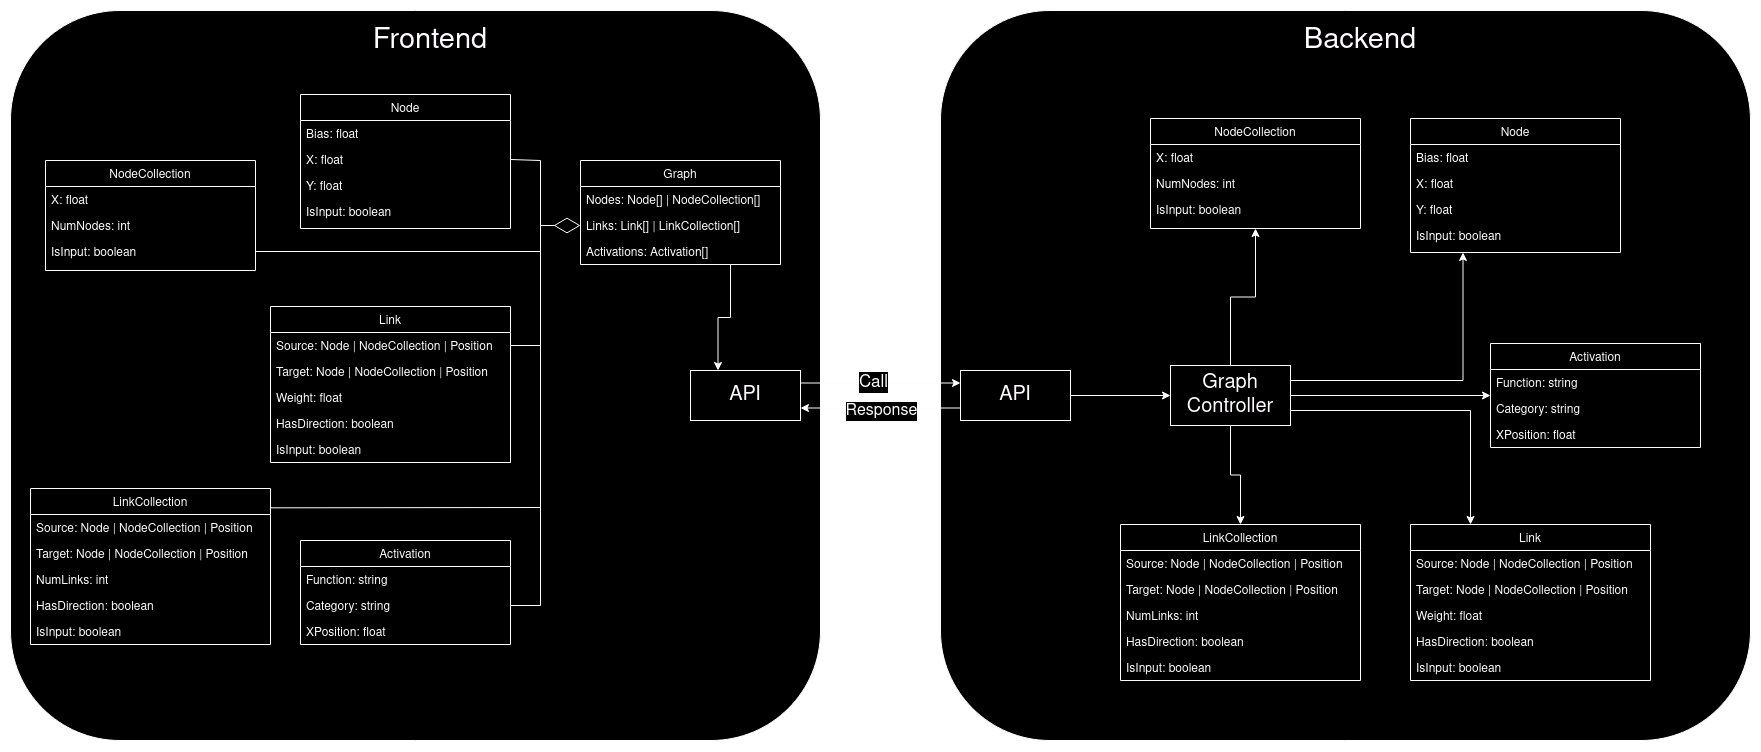
\includegraphics[width=0.8\textwidth]{../docs/diagrams/class_diagram.png}
    \caption{UML Class Diagram}
    \label{fig:uml_class_diagram}
\end{figure}

\subsubsection{Frontend/Client}
The frontend primarily relies on the Graph object, which is comprised of a number of Nodes and/or Node Collections, Links and/or Link Collections, and Activation Functions. Nodes represent individual nodes as represented in the graph, and these are used for nodes in graph layers that are smaller than 10 nodes by default. For layers that are too large, the graph representation instead contains a Node Collection that represents the layer as a whole. Links and Link Collections operate a similar way. Activation Function objects represent the activation functions that can be seen as small icons at the top of each layer in the NeuraViz interface. The graph object houses the representation of the neural network model as ready for rendering. As shown in the UML diagram, the frontend also houses an API component that is responsible for communicating with the backend architecture via standard HTTP requests.

\subsubsection{Backend/Server}
The backend is responsible for handling the computationally intensive processes of parsing the uploaded model and generating the structure of the visual representation. As seen in Figure \ref{fig:uml_class_diagram}, the backend houses objects that almost perfectly mirror the frontend components. However, on the server, these components are all related to the graph controller: the component responsible for the actual graph parsing. In addition to parsing the actual graph, the controller also handles additional requests for retrieving a stored model and converting the representation into various formats. Like with the frontend portion of the application, the backend houses an API component that is responsible for receiving the HTTP requests from the client and routing them to the correct controller endpoint for processing, as well as sending the response back to the client.

\subsection{Database}
At the outset of NeuraViz's development, no database was planned to be used. The nature of the application is such that the primary functionality of the application should not require a user to log in, and NeuraViz itself does not need to store information of any kind. Initially, the users' uploaded models get saved to disk during processing, but are then deleted immediately after for security and space efficiency. However, once the LaTeX export feature was introduced, it became necessary to maintain the graph's representation for longer, or to send it back and forth between the client more. Since the graph representation can be quite large, it was decided to use a NoSQL database, namely MongoDB, to store the parsed graph information as a session.

When a user makes their first request to the NeuraViz application, a session is created and the client is given an identifier. Upon graph parsing, the graph representation is stored in the database under the session identifier. Further requests can then retrieve the stored graph representation from the database, rather than having to re-upload the model and re-parse it. In addition to the LaTeX export feature, this also allows for the possible future features of saving the graph representation of a user's account for future reference, providing further granularity on larger networks, and more.

\subsection{User Interface}
A major step in the design process was developing the look and feel of the interface that users would be interacting with. A user interface mockup was drawn in Gimp to give a visual representation of what the application would look like. The mockup served as a guide in developing the actual user interface, though some changes were made to the final product. Since NeuraViz operates on a single page with one main piece of functionality, the required mockup was fairly simple. Figure \ref{fig:ui_mockup} shows a number of components that were included in the final product. The file upload button can be seen in the side panel on the left, along with its model validation text. Below that can be seen a section for settings with an example of what a setting with a slider might look like. While no final components use a slider so far, future development may include more complex settings. In addition to the sidebar, the primary visualization window can be seen with a sample model visualization. In the bottom right corner, navigation buttons can be seen in the mockup, mirroring the final interface.

\begin{figure}[h]
    \centering
    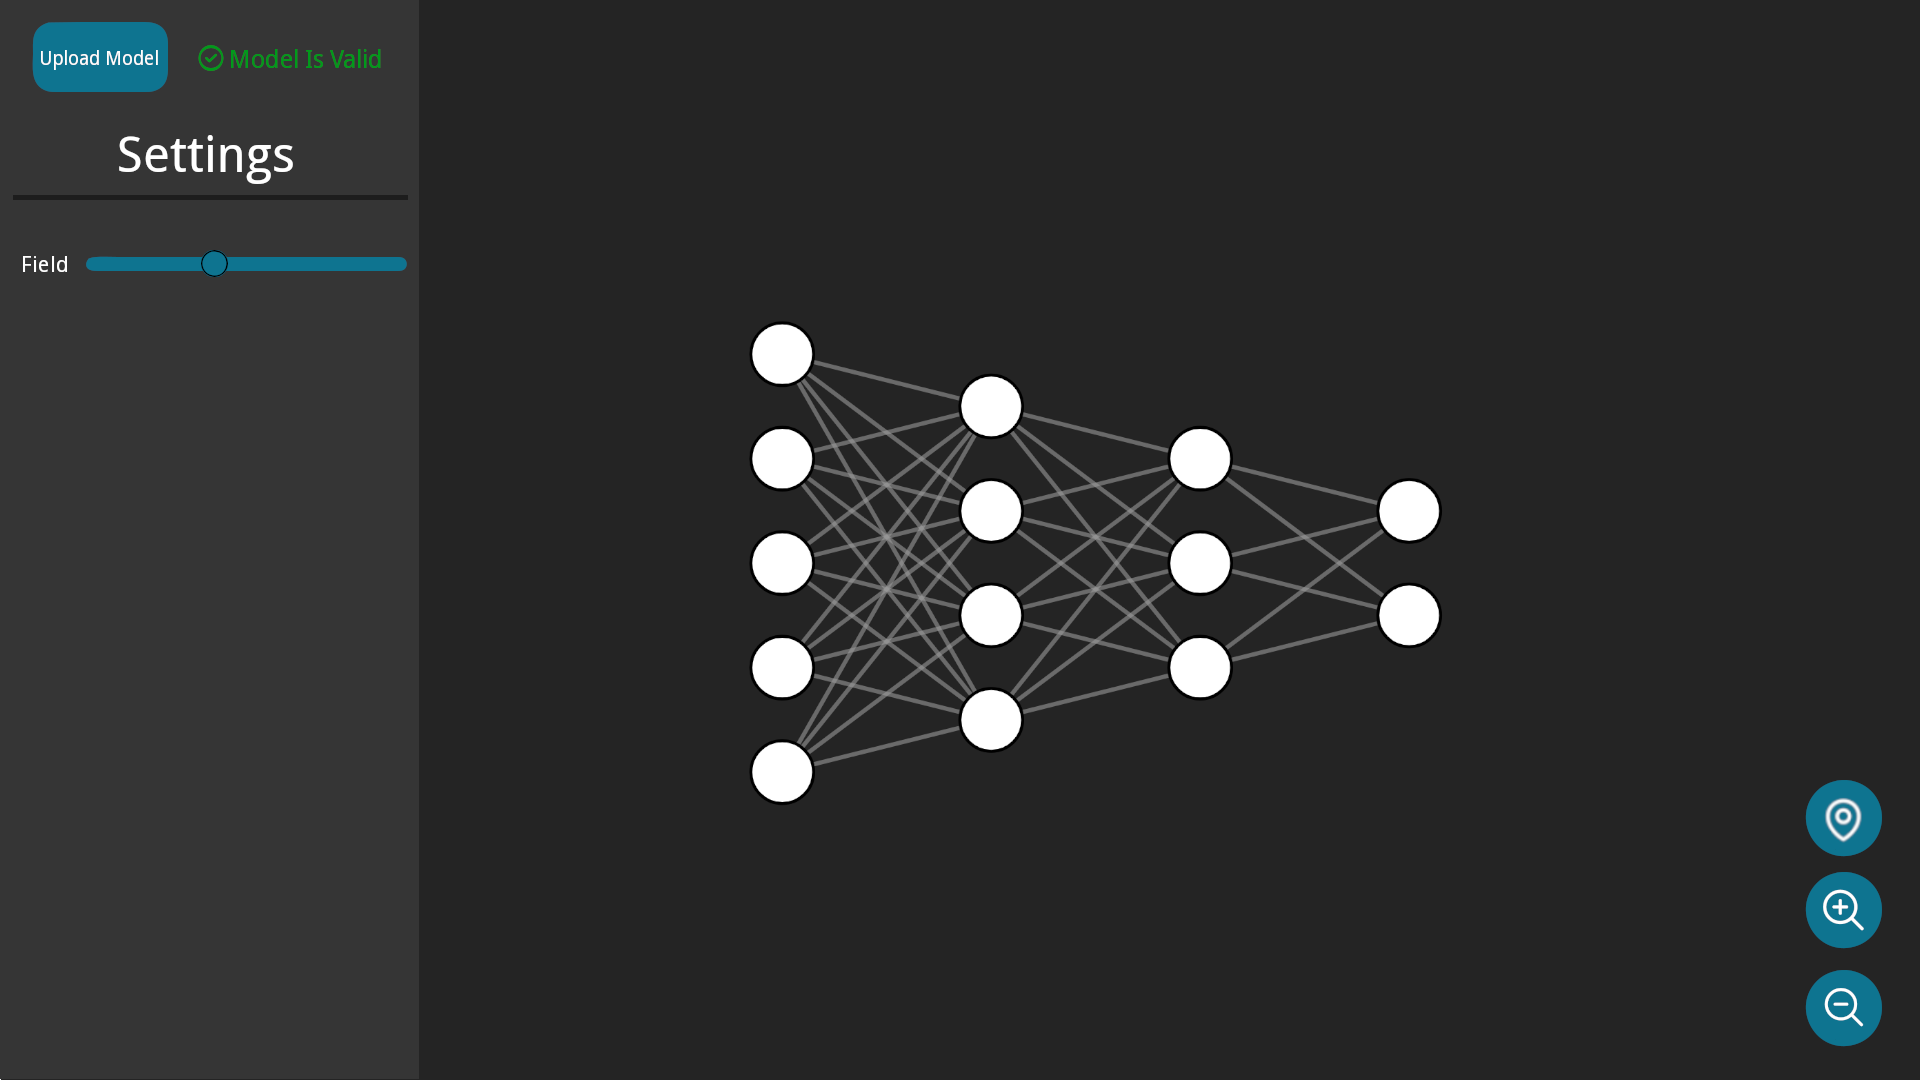
\includegraphics[width=1\textwidth]{../docs/mockups/Main.png}
    \caption{User Interface Mockup}
    \label{fig:ui_mockup}
\end{figure}

\subsubsection{Final Interface}
The final interface of NeuraViz is shown in Figure \ref{fig:ui_final}. The interface is divided into two main sections: the sidebar and the main visualization window. At the top of the sidebar, the file upload section can be seen, including a file picker, upload button, and model validation text. Below that, the options for visualization export can be seen, with buttons for both exporting the visualization to LaTeX and to SVG. Next the settings panel can be seen, with a mode toggle for the color scheme of the application. At the bottom of the sidebar there is a color reference key for the colors used in the main visualization window. 

The main visualization window contains the visualization of the model, or an indication that the user should upload a model. The colors of nodes and edges correspond to the color key found on the sidebar. Navigation buttons can be found at the bottom right of the page.

\begin{figure}[h]
    \centering
    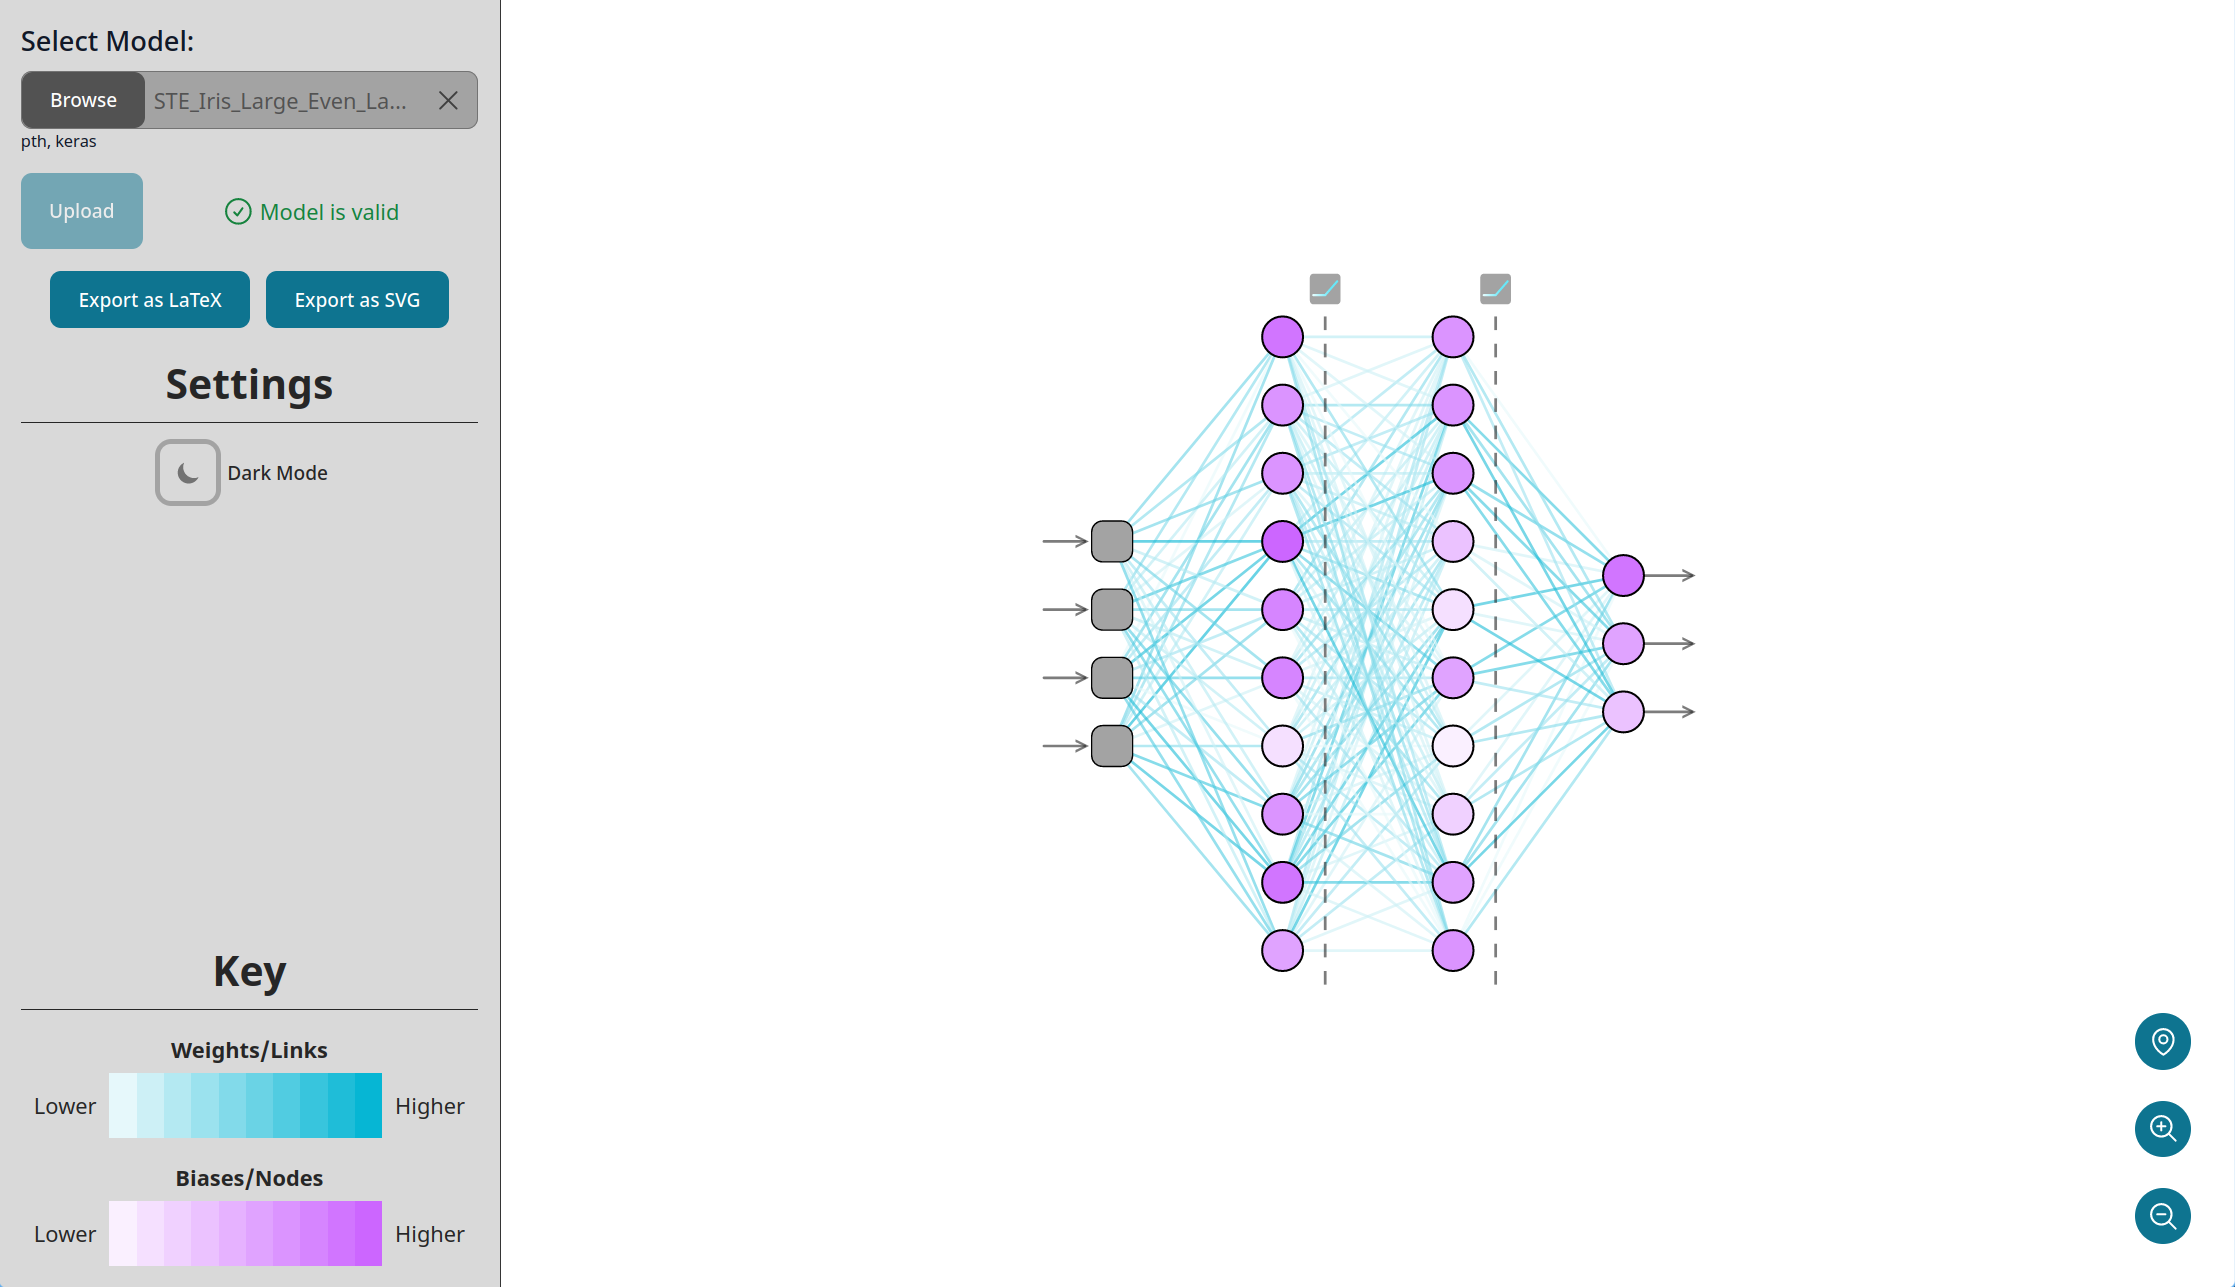
\includegraphics[width=1\textwidth]{03_design/res/final_interface.png}
    \caption{Final Interface}
    \label{fig:ui_final}
\end{figure}